%%% PGCON 2012
%%%
%%% Once a Top-10 internet audience site. 32 million users. Billions of
%%% photos and comments, more than 6TB of them. Migrating away from MySQL to
%%% PostgreSQL!
%%%
%%% This talk will share hindsights about the why and the how of that
%%% migration, what problems couldn't be solved without moving away and how
%%% the solution now looks. The tools used for migrating away the data, the
%%% methods and will detail the new architecture. And the new home, in the
%%% cloud!
%%%
%%% On the technical side of things, we will be talking about MySQL,
%%% mysqltocsv, pgloader, pljava, Google Protocol Buffers, pgbouncer,
%%% plproxy, PostgreSQL, pghashlib, walmgr, streaming replication. And
%%% Amazon hosting facilities too (EBS for starters).
%%%
%%%
%%%
%%% fotolog@admin=# select min(stat_day), max(stat_day), avg(nb_registration), avg(nb_photos_add), avg(nb_guestbook_add) from fl.stats_user_activity limit 35;
%%%    min     |    max     |          avg          |        avg         |        avg         
%%% ------------+------------+-----------------------+--------------------+--------------------
%%% 2012-03-02 | 2012-05-13 | 1309.3287671232876712 | 16046.890410958904 | 11046.452054794521
%%% (1 row)

\documentclass[english]{beamer}
\usepackage[utf8,latin9]{inputenc}
%%\usepackage[latin9]{inputenc}
\usepackage[T1]{fontenc}
\usepackage{babel}

\usepackage{beamerthemesplit}
%%\usetheme{Amsterdam}
\usetheme{Warsaw}
\beamertemplatetransparentcovered

\title{Large Scale MySQL Migration}
\subtitle{to PostgreSQL!}
\author{Dimitri Fontaine}
\date{May 17, 2012}

\begin{document}

\frame{\titlepage}

\section*{Agenda}
\frame{
  \frametitle{Content}
  \tableofcontents[pausesections]
}

\section{Fotolog}

\subsection{Presentation}

\frame{
  \frametitle{Fotolog}

  \begin{itemize}
   \item Photo Sharing website
   \item with friends and favorites
   \item \texttt{32 000 000} users
   \item \texttt{ 1 000 000 000} photos
   \item \texttt{10 000 000 000} comments
  \end{itemize}
}

\subsection{Former Architecture}

\frame{
  \frametitle{Former Architecture}

  Fotolog used to be a Java and MySQL shop:

  \begin{center} 
    \includegraphics[height=2.6in]{old_arch}
  \end{center} 
}

\subsection{A Wind of Change}

\frame{
  \frametitle{Why change?}

  We had to change, not mainly for technical reasons, mind you.

  \begin{itemize}
   \item<1-> Hi-Media acquired Fotolog in 2009
   \item<2-> Switched from \textit{Time to Market} to \textit{Rentability}
   \item<2-> Too costly, not making enough revenue
   \item<3-> Not reliable enough
   \item<4-> Founders not here anymore
   \item<5-> Knowledge of the application was gone
  \end{itemize}
}

\frame{
  \frametitle{Why PostgreSQL?}

  What else could we've been using after that? :)

  \begin{itemize}
   \item<1-> Hi-Media is a PostgreSQL shop
   \item<2-> Highly reliable, power all services
   \item<3-> Need to prepare for growth
   \item<4-> And keep the costs low
  \end{itemize}
}

\section{The new architecture}

\subsection{PostgreSQL Architecture}

\frame{
  \frametitle{Current Architecture, part 1/2}

  Hi-Media is a PHP shop, for what it's worth, and manages to still be
  reliable thanks to PostgreSQL, used on the front servers:

  \begin{center} 
    \includegraphics[height=2.4in]{new_arch_web}
  \end{center} 
}

\frame{
  \frametitle{Current Architecture, part 2/2}

  And on the data servers too, of course:

  \begin{center} 
    \includegraphics[height=2.1in]{new_arch_db}
  \end{center} 
}

\begin{frame}[fragile]
  \frametitle{\texttt{PL/Proxy}}

  \textit{pl/proxy} is the integrated sharding layer. Now you have to write
  all your SQL in server side functions.

  \begin{example}[admin/change\_group\_status.sql]
\begin{verbatim}
create or replace function admin.change_group_status
(
    user_name text, status integer
)
returns void as $BODY$
    CLUSTER 'fl_cluster';
    RUN ON hash_string(user_name, 'lookup3le');
$BODY$;
\end{verbatim}
  \end{example}
\end{frame}

\section{The Migration}

\subsection{Code}

\frame{
  \frametitle{Migrating the Code. Wait, WAT?}

  Keeping the old Java code base that was halfway through a complete rewrite
  in Scala... could have been an option. But

  \begin{itemize}
   \item The goal here is to get knowledge back
   \item Noone deals with Java
   \item Small enough set of features
   \item Complete rewrite in PHP / plproxy
  \end{itemize}
}

\subsection{Services}

\frame{
  \frametitle{Amazon Hosting}

  The new platform is all at Amazon, and we had to have something cheap
  enough so as to maximize the revenues from the website:

  \begin{itemize}
   \item<1-> Web server, EC2, 8GB RAM, 8 CPU, 16 of them
   \item<1-> Database servers, EC2, 15GB RAM, 4*400GB local disks
   \item<1-> 16 database servers, each hosting 16 databases shards
   \item<2-> Cron server, web like, admin server, bdd like
   \item<3-> Backup server, EC2, 15GB RAM, 18 EBS (500GB), 18 Hot Standbies
   \item<3-> S3 storage for archiving (WAL-E)
  \end{itemize}
}

\frame{
  \frametitle{Migrating the Services}

  When migrating from an old to a new platform it can get tricky if you
  can't replace the hardware while at it.

  \begin{itemize}
   \item Former hosting was judged too costly
   \item New hosting needed, hard to scale properly
   \item Amazon Web Services, here we go
   \item New Hosting means for easier switchover
  \end{itemize}
}

\subsection{Data}

\frame{
  \frametitle{Foreign Data Wrappers}

  We first tried some fancy newer stuff.

  \begin{itemize}
   \item<1-> Streaming data from MySQL to PostgreSQL?
   \item<1-> using the MySQL Foreign Data Wrapper
   \item<2-> did have to edit the code
   \item<3-> very very slow rate
   \item<3-> even after optimization tries
  \end{itemize}
}

\frame{
  \frametitle{pipe \texttt{mysql} to \texttt{pgsql}}

  Back to the basics then.

  \begin{itemize}
   \item<1-> \texttt{echo \$sql| mysql| psql}
   \item<2-> MySQL man page pretends to be sending CSV
   \item<2-> But that's a lie.
   \item<3-> so we had to write a very simple \texttt{mysql2csv} client
   \item<3-> and summon \texttt{pgloader} to the rescue!
  \end{itemize}
}

\frame{
  \frametitle{Data migration}

  So we ended up with a complex enough data migration script set:

  \begin{center} 
    \includegraphics[height=1.3in]{data_migration}
  \end{center} 
}

\frame{
  \frametitle{Data migration}

  Some details about that migration scripts:

  \begin{itemize}
   \item<1-> 37 different mysql sources
   \item<2-> loading to temp PostgreSQL where it's all text
   \item<3-> \texttt{COPY OUT} from a query with lots of \texttt{COALESCE}
   \item<3-> that's where we process \texttt{0000-00-00} dates and the like
   \item<4-> oh, and \textit{blobs} too
  \end{itemize}
}

\subsection{Blobs}

\frame{
  \frametitle{Did I head \textit{Binary data}?}

  Yes you did.

  \begin{itemize}
   \item<1-> MySQL made it complex to adapt the schema live
   \item<1-> and to partition data (13 times the same guestbook table)
   \item<2-> finally they opted for \textit{Google Protocol Buffers}
   \item<2-> the API is available for Java, C++ and Python
   \item<2-> we tried \texttt{pl/python} first, encoding and \texttt{NULL} problems
   \item<3-> we then tried \texttt{pl/java}
  \end{itemize}
}

\begin{frame}[fragile]
  \frametitle{Did I head \textit{PL/Java}?}

  \begin{example}[jblobs.sql]
\begin{verbatim}
CREATE TYPE public.gb_message_t
  AS (is_private boolean, parent_id int4,
      msg text, user_name text);

CREATE OR REPLACE FUNCTION
     public.decode_guestbook_message (in bytea)
  RETURNS public.gb_message_t
  AS 'com.fotolog.blob.GuestBook.getMessage'
  STRICT IMMUTABLE LANGUAGE java;
\end{verbatim}
  \end{example}
\end{frame}

\begin{frame}[fragile]
  \frametitle{Did I head \textit{PL/Java}? (twice now)}

  \begin{example}[src/com/fotolog/blob/GuestBook.java]
\begin{verbatim}
package com.fotolog.blob;
import java.sql.ResultSet;
import com.fotolog.proto.fl.Fl;

class GuestBook {
    public static boolean
       getMessage(byte[] blob, ResultSet receiver) throws Exception
    {
	try {/* see next slide */}
	catch( Exception e ) {return false; /* NULL */}
    }
}
\end{verbatim}
  \end{example}
\end{frame}

\begin{frame}[fragile]
  \frametitle{Did I head \textit{PL/Java}? (ok, last time)}

  \begin{example}[src/com/fotolog/blob/GuestBook.java]
\begin{verbatim}
	    Fl.GuestbookMessage mess =
	    	    Fl.GuestbookMessage.parseFrom(blob);
	    Fl.GuestbookMessageV1 v1 = mess.getV1();

	    receiver.updateBoolean(1, v1.getIsPrivate());
	    receiver.updateLong(2, v1.getParentId());
	    receiver.updateString(3, v1.getMsgTxt());
	    receiver.updateString(4, v1.getPostedBy());

	    return true;
\end{verbatim}
  \end{example}
\end{frame}

\section{Conclusion}

\subsection{In production}

\frame{
  \frametitle{Still growing}

  The community has been following us in the new setup, we still see some
  activity:

  \begin{itemize}
   \item \texttt{ 1310} new users a day, average
   \item \texttt{ 4375} new friends a day, average
   \item \texttt{16046} new photos a day, average, maxing out at \texttt{93840}
   \item \texttt{11046} new comments a day, average
  \end{itemize}
}

\frame{
  \frametitle{Activity in graphs 1/7}

  Let's see about activity in term of munin graphs. PGQ:

  \begin{center} 
    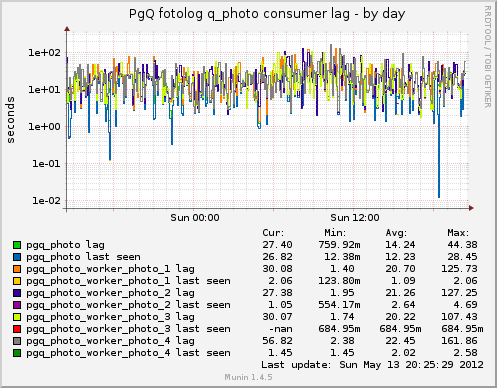
\includegraphics[height=2.1in]{pg_queue_fotolog_q_photo-day.png}
  \end{center} 
}

\frame{
  \frametitle{Activity in graphs 2/7}

  I love \texttt{pgbouncer} graphs, here are the db clients:

  \begin{center} 
    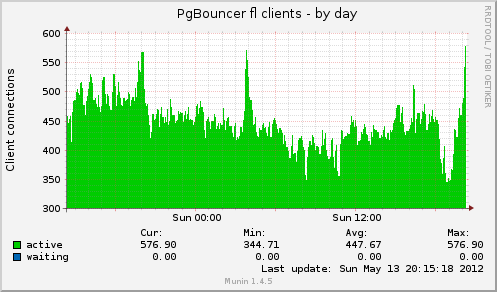
\includegraphics[height=2.1in]{pgbouncer_db_fl_pools_cl-day}
  \end{center} 
}

\frame{
  \frametitle{Activity in graphs 3/7}

  And the server sessions to serve them (\texttt{447} average):

  \begin{center} 
    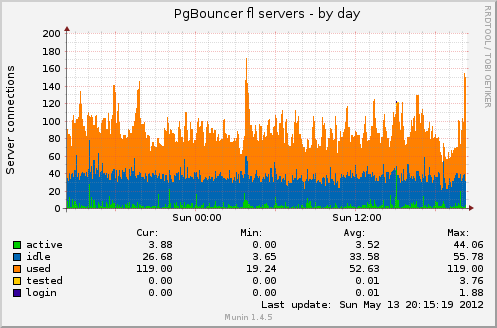
\includegraphics[height=2.1in]{pgbouncer_db_fl_pools_sv-day}
  \end{center} 
}

\frame{
  \frametitle{Activity in graphs 4/7}

  \texttt{pgbouncer} even maintains query length speed stats:

  \begin{center} 
    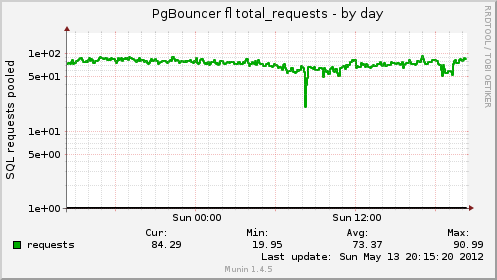
\includegraphics[height=2.1in]{pgbouncer_db_fl_stats_requests-day}
  \end{center} 
}
\frame{
  \frametitle{Activity in graphs 5/7}

  Now, processed transactions on db nodes:

  \begin{center} 
    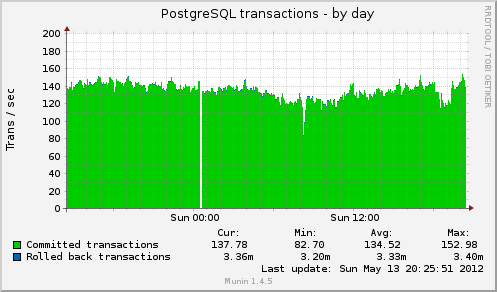
\includegraphics[height=2.1in]{postgres_db_transactions_ALL-day}
  \end{center} 
}

\frame{
  \frametitle{Activity in graphs 6/7}

  And processed transactions on proxy nodes (those web servers):

  \begin{center} 
    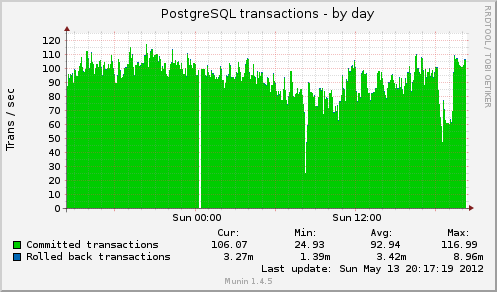
\includegraphics[height=2.1in]{postgres_web_transactions_ALL-day}
  \end{center} 
}

\frame{
  \frametitle{Activity in graphs 7/7}

  Finally, spot the problem here:

  \begin{center} 
    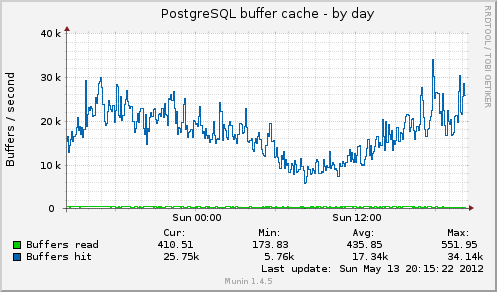
\includegraphics[height=2.1in]{postgres_db_cache_ALL-day}
  \end{center} 
}

\subsection{Any question?}

\frame{
  \frametitle{Any question?}

  \begin{center}
    Now is a pretty good time to ask!
  \end{center}
}

\end{document}
